\exercise

Apply the ``binary search with exponential jumps'' (a.k.a. galloping search, or
doubling algorithm) to the search of the item 51 within the sorted sequence: $$S
= [\,2,\ 4,\ 6,\ 7,\ 15,\ 23,\ 24,\ 25,\ 28,\ 31,\ 51,\ 90,\ 92,\ 101,\ 130,\
131,\ 150,\ 189\,].$$

\solution

\autoref{fig:doubling} shows the execution of the doubling search on the
provided sequence. First, the exponential jumps find the delimiters of the
subsequence such that $S[i + 2^{k-1}] < 51 \le S[i + 2^k]$ (in this case, $i =
0$). Then we search 51 on that subsequence with a classical binary search.
%
\begin{figure}[bh]
  \centering
  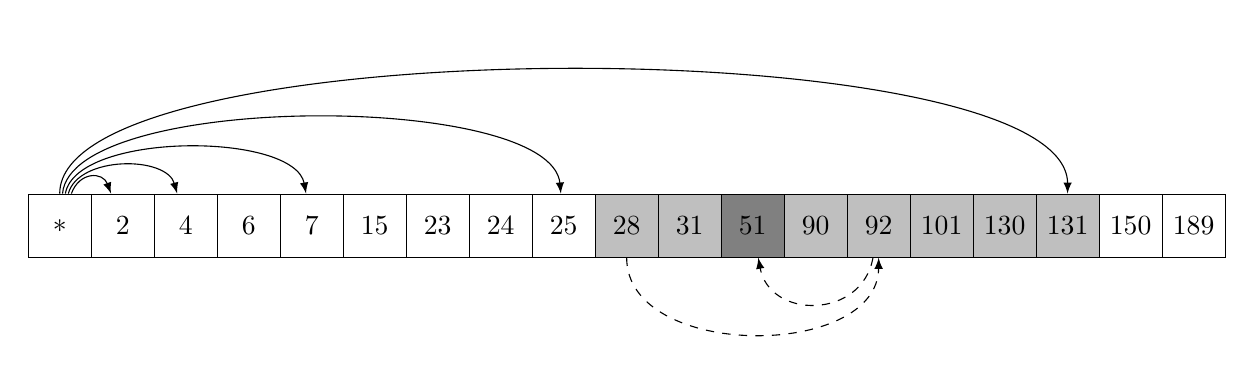
\begin{tikzpicture}[
      node distance=0.8cm,
      every node/.append style={
        draw,rectangle,
        minimum width=0.8cm,
        minimum height=0.8cm,
        inner sep=0
      }
    ]

    \node[fill=white] (0) {$\textasteriskcentered$};
    \node[right of=0, fill=white] (1) {2};
    \node[right of=1, fill=white] (2) {4};
    \node[right of=2, fill=white] (3) {6};
    \node[right of=3, fill=white] (4) {7};
    \node[right of=4, fill=white] (5) {15};
    \node[right of=5, fill=white] (6) {23};
    \node[right of=6, fill=white] (7) {24};
    \node[right of=7, fill=white] (8) {25};
    \node[right of=8, fill=lightgray] (9) {28};
    \node[right of=9, fill=lightgray] (10) {31};
    \node[right of=10, fill=gray] (11) {51};
    \node[right of=11, fill=lightgray] (12) {90};
    \node[right of=12, fill=lightgray] (13) {92};
    \node[right of=13, fill=lightgray] (14) {101};
    \node[right of=14, fill=lightgray] (15) {130};
    \node[right of=15, fill=lightgray] (16) {131};
    \node[right of=16, fill=white] (17) {150};
    \node[right of=17, fill=white] (18) {189};

    \path (0) edge[-latex, out=70, in=110, distance=0.3cm] (1);
    \path (0) edge[-latex, out=75, in=105, distance=0.5cm] (2);
    \path (0) edge[-latex, out=80, in=100, distance=0.8cm] (4);
    \path (0) edge[-latex, out=85, in=95, distance=1.3cm] (8);
    \path (0) edge[-latex, out=90, in=90, distance=2.1cm] (16);

    \path (9) edge[dashed, -latex, out=-90, in=-90, distance=1.3cm] (13);
    \path (13) edge[dashed, -latex, out=-100, in=-80, distance=0.8cm] (11);

  \end{tikzpicture}

  \caption{Doubling search executed on the given sequence. Solid lines represent
  the steps of the exponential jumps, while dashed lines the ones of the binary
  search, which is performed over the gray subsequence. The leading asterisk is
  used just for visualization purposes: in a real doubling search (set
  intersection), it would have been the last returned (intersected) item.}

  \label{fig:doubling}
\end{figure}
